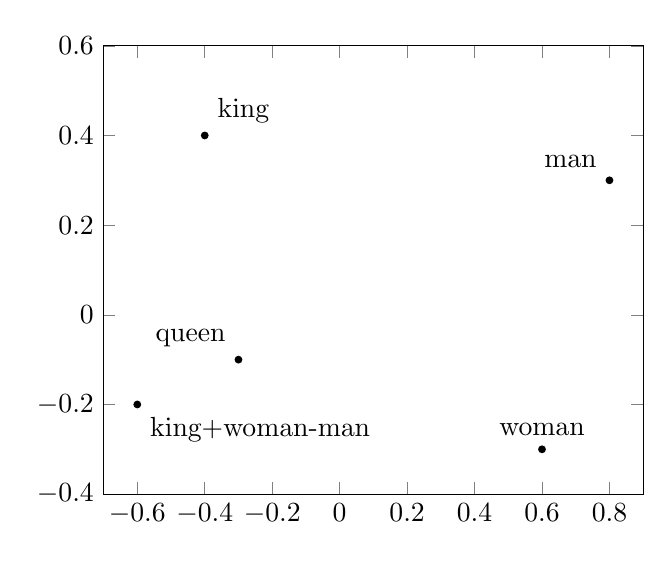
\begin{tikzpicture}
    \begin{axis}[
            xmin=-0.7,
            xmax=0.9,
            ymin=-0.4,
            ymax=0.6,
        ]
        \node[label={-45:{king+woman-man}},circle,fill,inner sep=1pt] at (-.6,-.2) {};
        \node[label={45:{king}},circle,fill,inner sep=1pt] at (-.4,.4) {};
        \node[label={90:{woman}},circle,fill,inner sep=1pt] at (.6,-.3) {};
        \node[label={135:{man}},circle,fill,inner sep=1pt] at (.8,.3) {};
        \node[label={135:{queen}},circle,fill,inner sep=1pt] at (-.3,-.1) {};
    \end{axis}
\end{tikzpicture}